%%%%%%%%%%%%%%%%%%%%% chapter.tex %%%%%%%%%%%%%%%%%%%%%%%%%%%%%%%%%
%
% sample chapter
%
% Use this file as a template for your own input.
%
%%%%%%%%%%%%%%%%%%%%%%%% Springer-Verlag %%%%%%%%%%%%%%%%%%%%%%%%%%
%\motto{Use the template \emph{chapter.tex} to style the various elements of your chapter content.}
\chapter{Execution Time and Analysis}
\label{Introduction}
The interest of this study was to analyse the execution times of the three algorithms described above, to determine which method executes in the fastest time and might be most appropriate for using to solve large problems. The execution times were measured for each method for domains of the following sizes with a maximum frequency of 500Hz for FDTD, SFDTD and PSTD in 3D:\\
\begin{center}
\begin{tabular}{|c|c|c|c|} 
  \hline
 Dimension ($m^3$) & FDTD Cells & SFDTDCells & PSTD Cells \\
 \hline
 5 & 121104	& 121104 & 24025\\ 
 10 & 483025 & 483025 & 62500\\  
 20 & 1932100 & 1932100 & 192721\\ 
 40 & 7722841 & 7722841 & 667489\\ 
 60 & 30880249 & 30880249 & 2474329\\ 
 \hline
\end{tabular}\\
\end{center}

The time step execution time was evaluated for 2000 executions, allowing for smaller or larger required time steps to be part of the analysis. The execution of each time step includes only the steps outlined above, with no plotting. Execution time was measured using Matlab internal timers. During execution, Matlab was the only task running in the foreground of the system, but background tasks were allowed to continue without restriction. The computer system used for these tests had the following properties:\\

\begin{itemize}
\item Intel Core i5 4690k CPU @ 4.5GHz @ 1.227V
\item 16GB DDR3 RAM @ 3875.3MHz
\item Asus Gryphon Motherboard with Z97 Chip Set
\end{itemize}

\section{Results}
The mean time step execution time for each method is given below in two bar charts, one with a linear and one with a logarithmic y axis: \\
\begin{figure}[H]
\centering
	\textbf{Mean Timestep Execution Speed with Log Axis}
  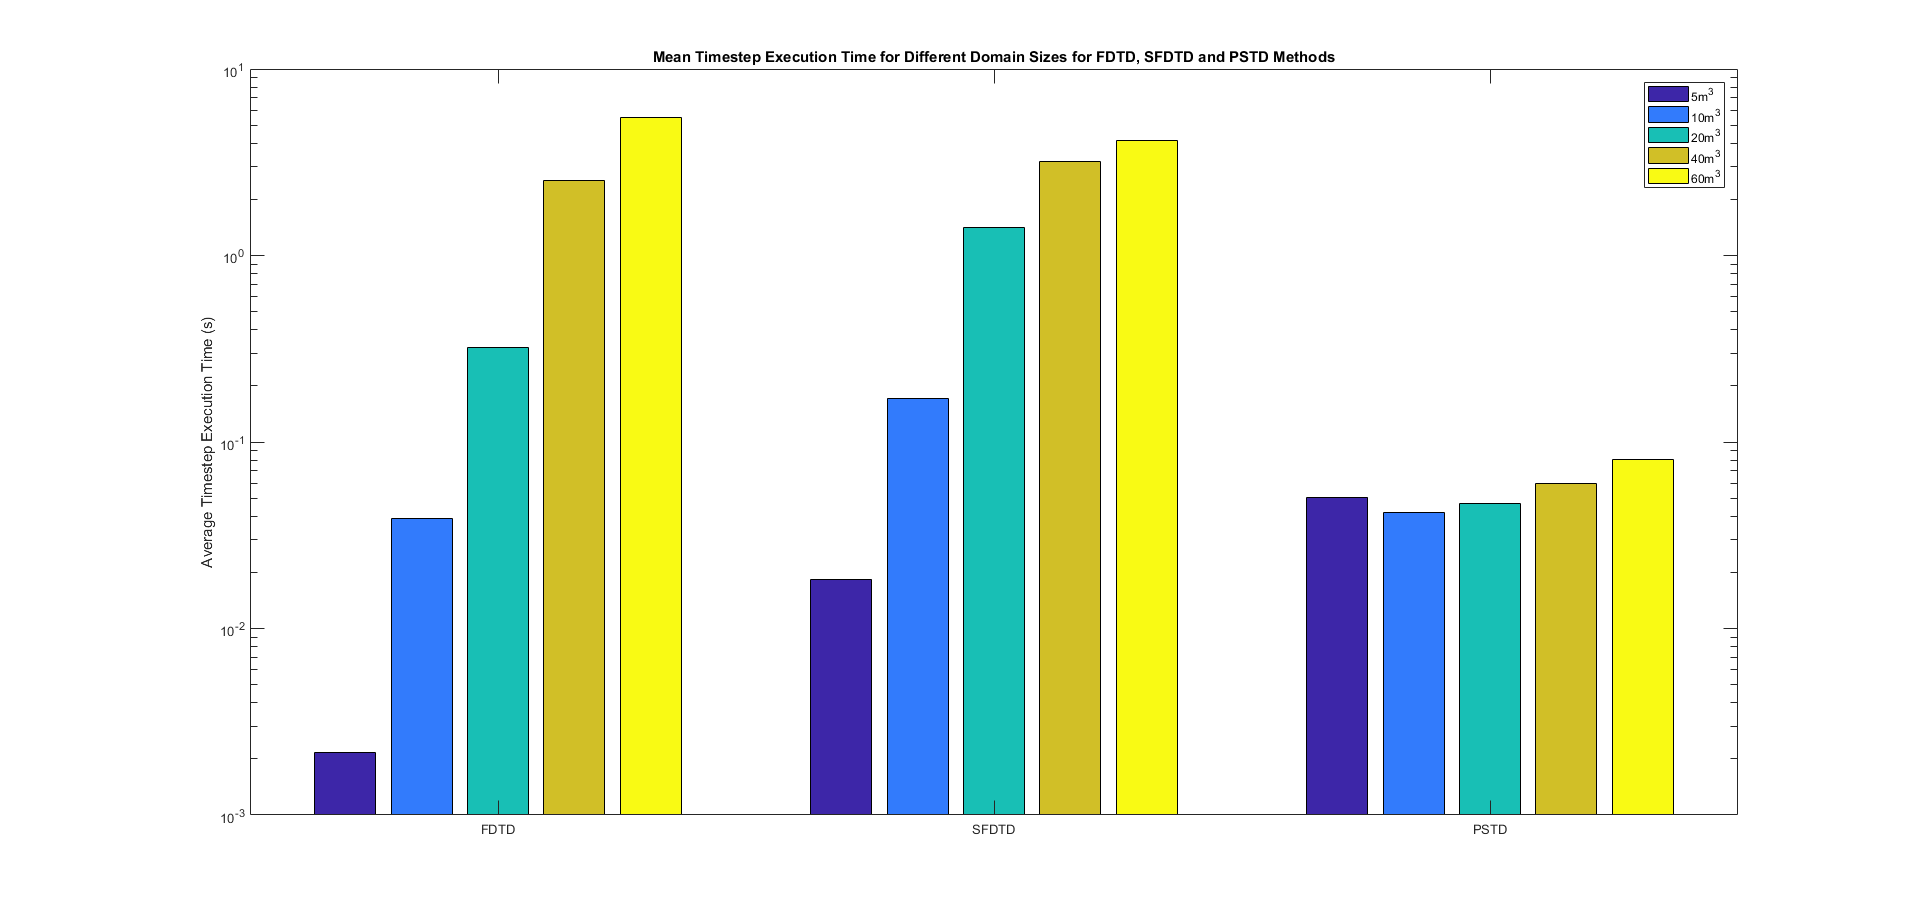
\includegraphics[width=\textwidth]{./graphics/speedTestBar.png}
  \caption{Execution times for FDTD simulations in domains of increasing size}
\end{figure}
\begin{figure}[H]
\centering
\textbf{Mean Timestep Execution Speed with Linear Axis}
  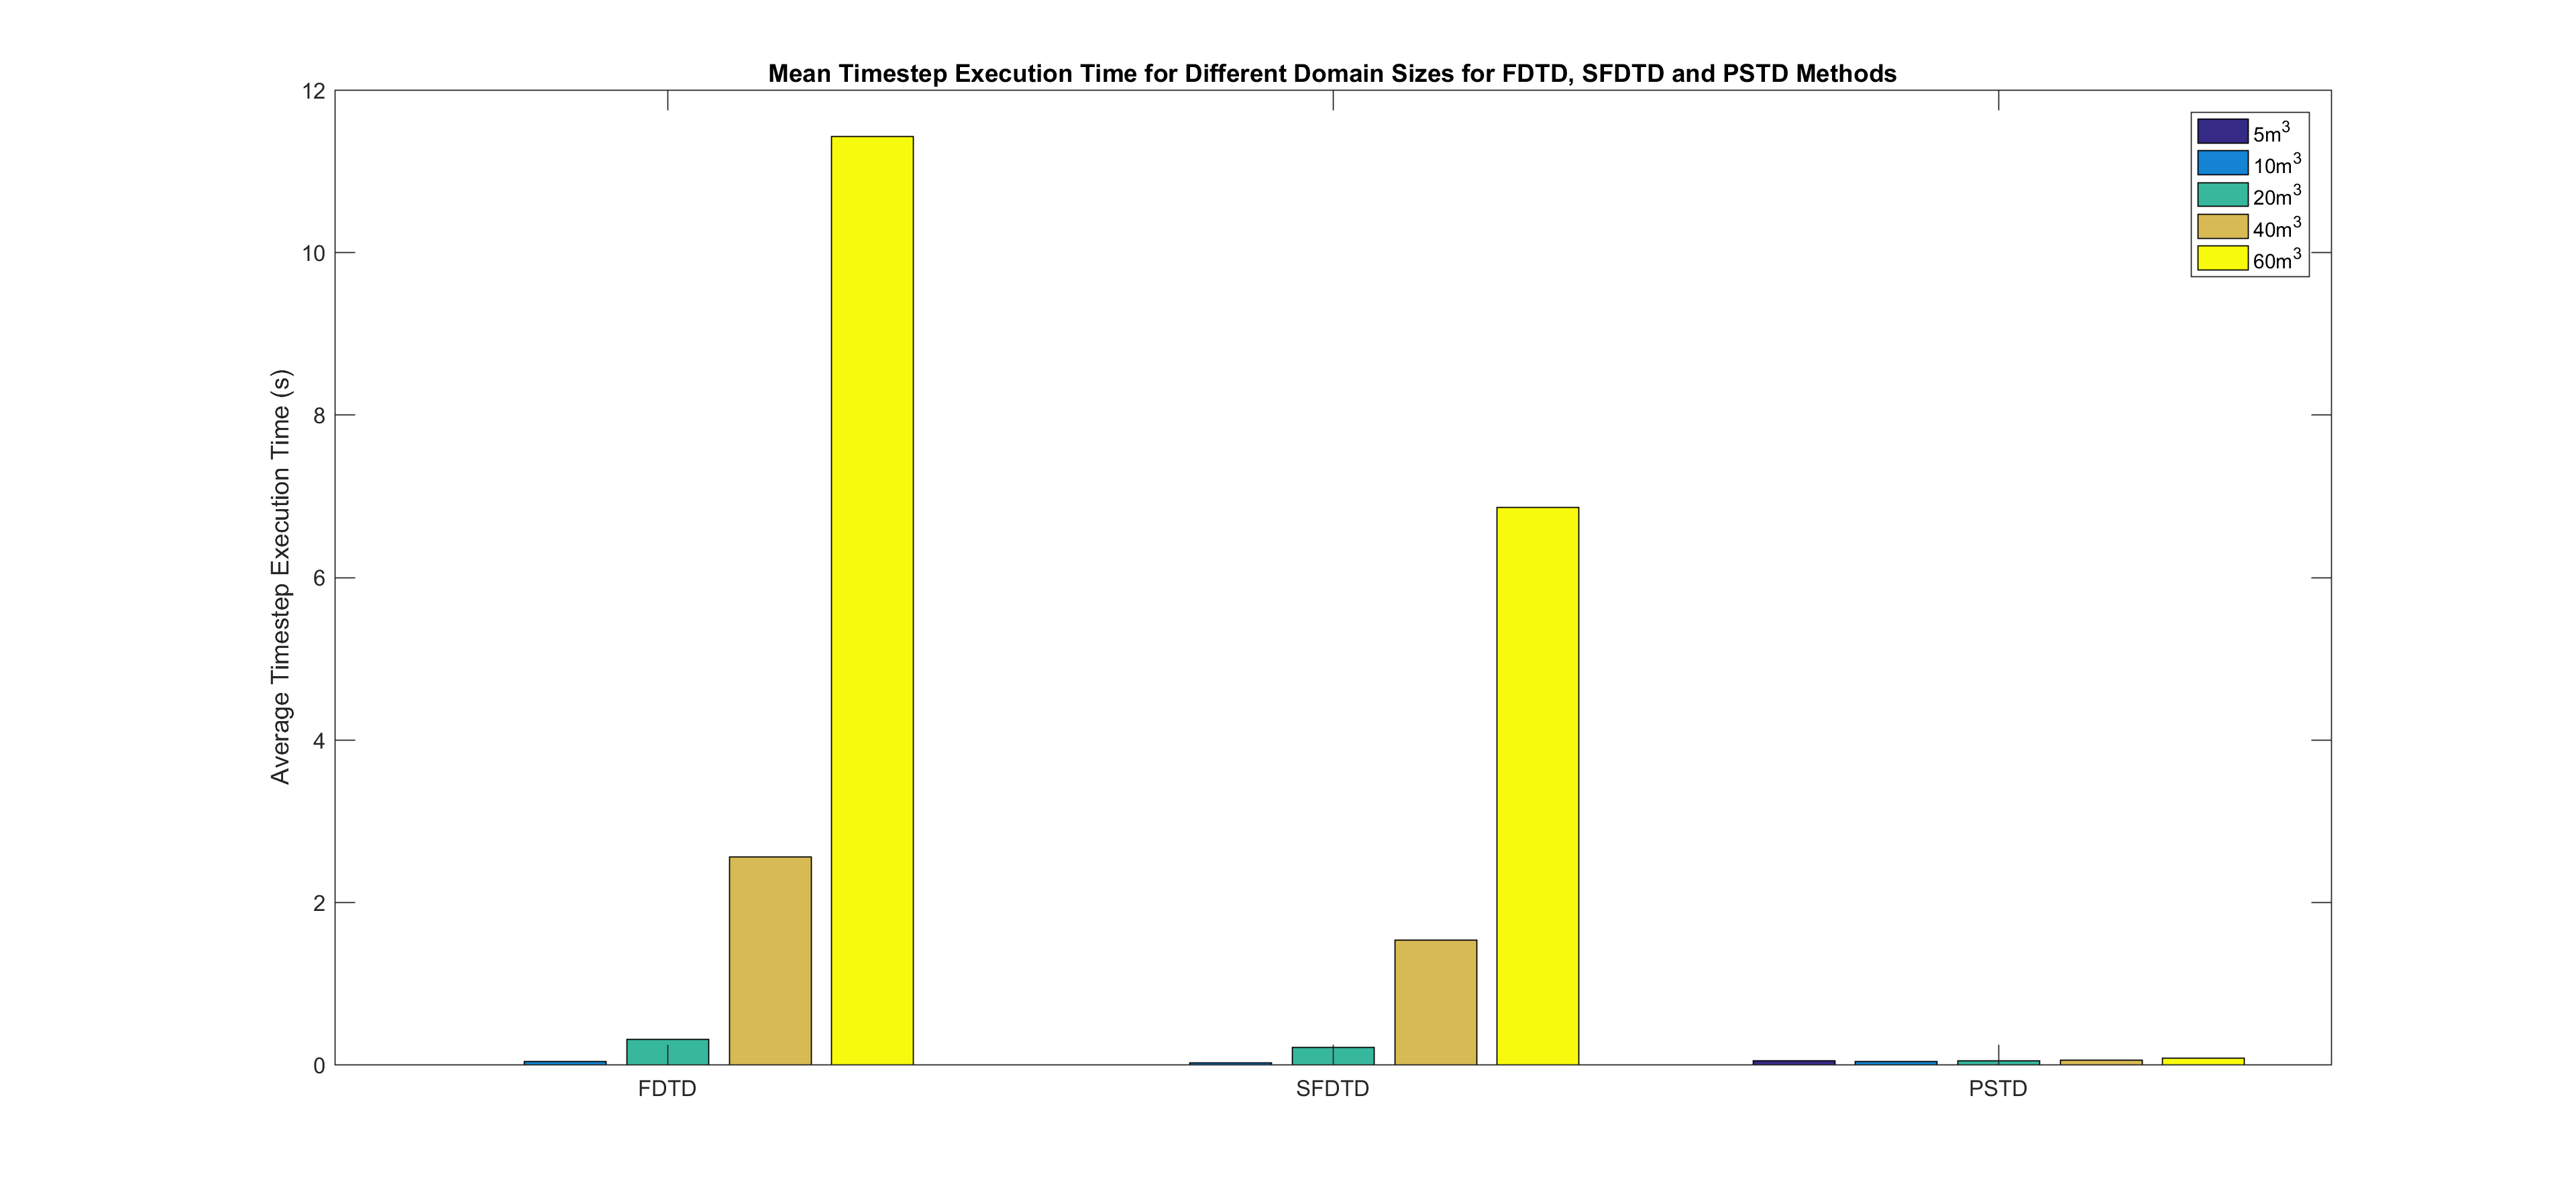
\includegraphics[width=\textwidth]{./graphics/speedTestBarlin.png}
  \caption{Execution times for FDTD simulations in domains of increasing size}
\end{figure}

\section{Analysis}

These results show the scale of the increase in execution speed with domain size. Both the FDTD and SFDTD methods average timestep execution speed increase exponentially with domain size, where the PSTD method shows a minimal increase in execution time. Though not shown by this data, the aggregate execution time of the FDTD simulation for a $40m^3$ domain was 1 hour 5 minutes. Where as execution for the same domain in PSTD was 1.5 minutes. This data suggests that the PSTD method executes significantly faster for larger domains than the FDTD method. This is likely due to three main reasons: \\
\begin{itemize}
\item Differentiation in the frequency domain allows large domains to be evaluated fast, as many cells are differentiated at once.
\item The speed of the Fourier transforms is sufficiently fast to have little increase as the number of cells increases. 
\item Due to the nature of frequency domain differentiation, fewer cells are required per wavelength for stable simulation.
\end{itemize}
However as shown in the validation section the quality of the results of the PSTD method may be questionable, and it may be that a greater number of spatial steps and a reduced time step is required for improved results quality from the PSTD method. Further study of a Chebyshev PSTD method may help with this. The SFDTD method improves average execution speed, and gives results similar in quality to the FDTD method, and so may be worth further investigation and optimisation.
\section{Code Profiling}
Use of Matlabs code profiling tool analysis the performance of the PSTD3Dfun function shows the time taken for execution for 2000 calls of the function during an example simulation of a 5m by 4m by3m domain with a maximum frequency of 5kHz:\\
\begin{figure}[H]
\centering
  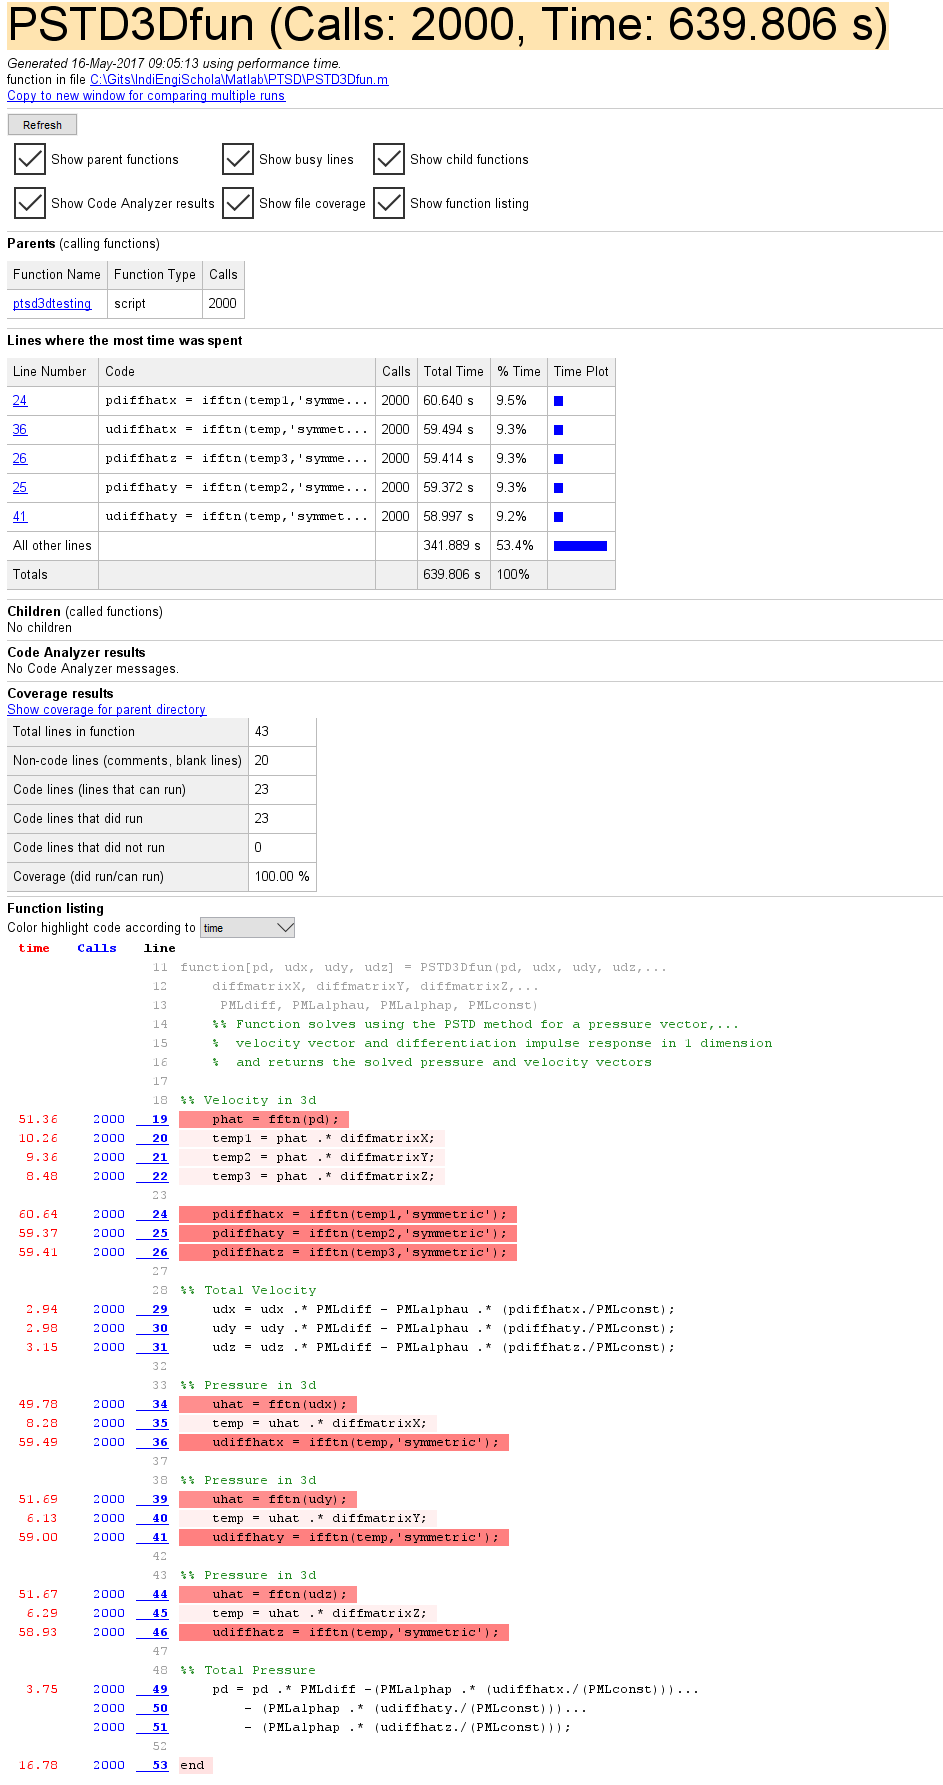
\includegraphics[width=\textwidth]{./graphics/pstdfunctioncodeprofile.png}
  \caption{Code execution time profile of PSTD functions}
\end{figure}
This shows that most time in the execution was spent performing the IFFT of the 3D matrices, and that the maximum average differentiation time was 5.1ms for a matrix of 80724 points in the x direction. Below is a figure showing the code profiling for 1200 calls of the FDTD3Dfun function for an example simulation of a 5m by 4m by3m domain with a maximum frequency of 1kHz:\\
\begin{figure}[H]
\centering
  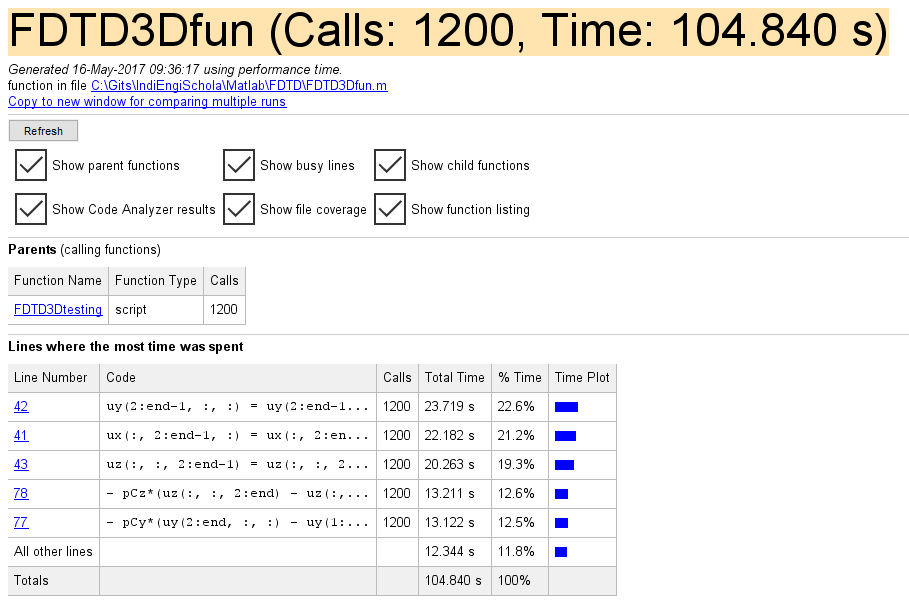
\includegraphics[width=\textwidth]{./graphics/fdtdfunctioncodeprofile.png}
  \caption{Code execution time profile of FDTD functions}
\end{figure}

These profiling results show that the bulk of the time spent in execution of the FDTD3Dfun function is used in the differentiation of the matrices. Combined with the total execution speed results for different domains above, the conclusion can be drawn that spectral differentiation may be more appropriate for large domains than finite or local differentiation. As the SFDTD method appears above to converge after some time to a uniform excution time, PSTD may be a more appropriate choice for further development of time domain numerical simulation in large domains. This however may not be a fair conclusion to draw against the SFDTD method as it is not implemented in 3D, further study is required to confirm the efficiency difference between PSTD and SFDTD.

The figure below shows a summary of the code profiling information for an SFDTD simulation of a 5m by 4m domain with maximum frequency of 1kHz, executing for $0.2s$:\\
\begin{figure}[H]
\centering
%  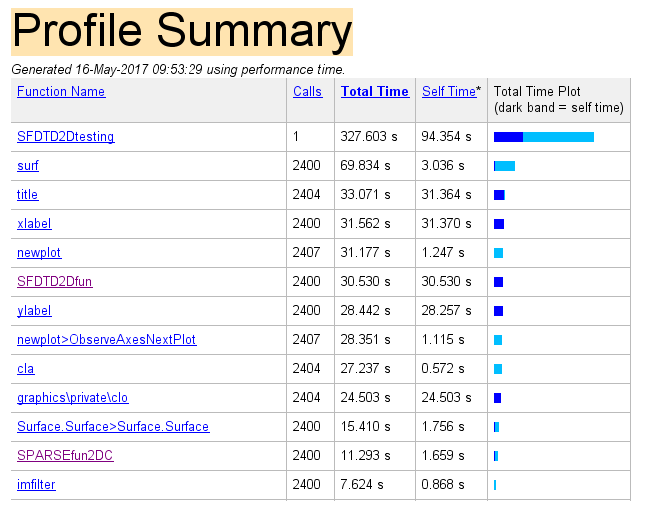
\includegraphics[width=1\textwidth]{./graphics/sfdtdprosum.png}
  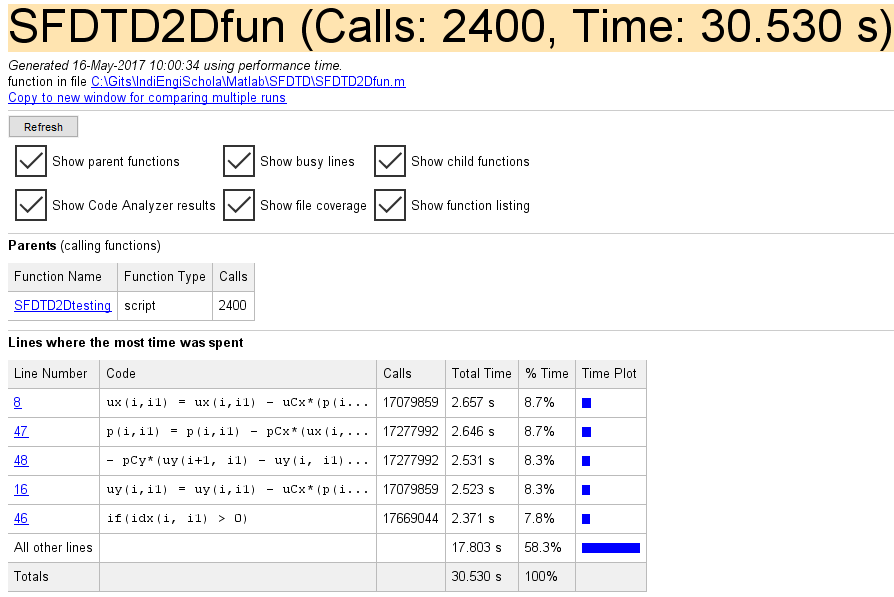
\includegraphics[width=1\textwidth]{./graphics/sfdtdfunprosum.png}
  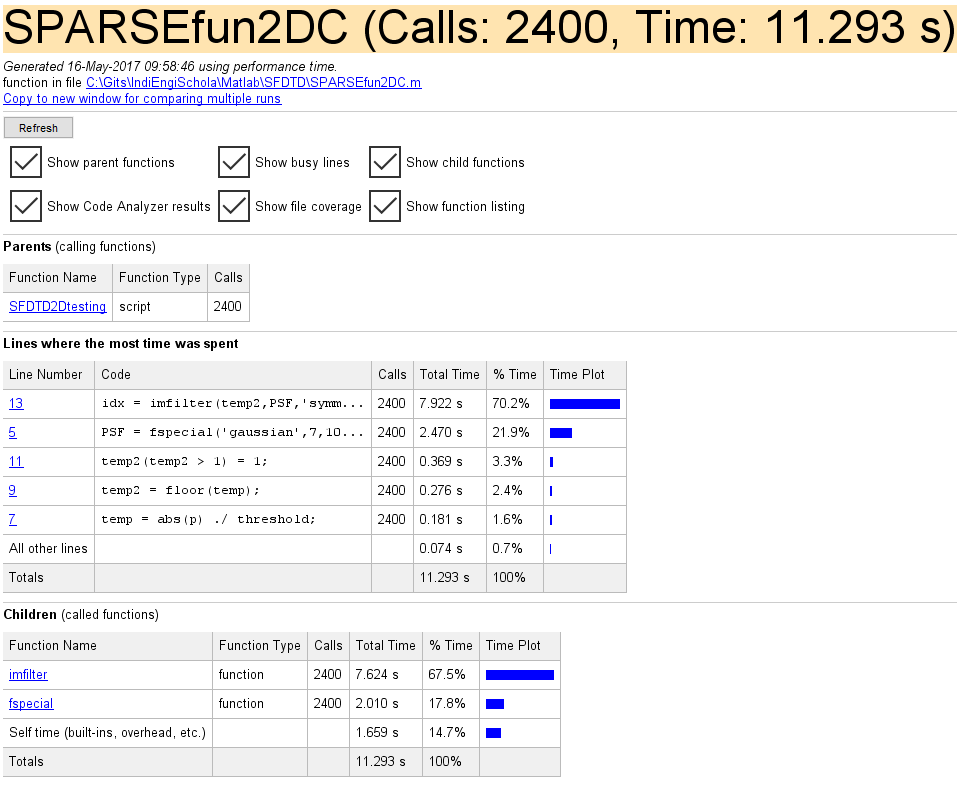
\includegraphics[width=1\textwidth]{./graphics/sparfunprosum.png}
  \caption{Code execution time profile of SFDTD functions}
\end{figure}
These results show that in the SFDTD method most time is spent differentiating the matrices as opposed to filtering the domain, although an extra process has been added that process does not take longer than the longest process in the original method. However, further study could provide a more optimal 3D filtering method for index matrix generation, as the function used for the smoothing is one designed by Mathworks for smoothing MRI data.
